\documentclass[twoside]{book}

% Packages required by doxygen
\usepackage{fixltx2e}
\usepackage{calc}
\usepackage{doxygen}
\usepackage[export]{adjustbox} % also loads graphicx
\usepackage{graphicx}
\usepackage[utf8]{inputenc}
\usepackage{makeidx}
\usepackage{multicol}
\usepackage{multirow}
\PassOptionsToPackage{warn}{textcomp}
\usepackage{textcomp}
\usepackage[nointegrals]{wasysym}
\usepackage[table]{xcolor}

% NLS support packages
\usepackage[spanish]{babel}
% Font selection
\usepackage[T1]{fontenc}
\usepackage[scaled=.90]{helvet}
\usepackage{courier}
\usepackage{amssymb}
\usepackage{sectsty}
\renewcommand{\familydefault}{\sfdefault}
\allsectionsfont{%
  \fontseries{bc}\selectfont%
  \color{darkgray}%
}
\renewcommand{\DoxyLabelFont}{%
  \fontseries{bc}\selectfont%
  \color{darkgray}%
}
\newcommand{\+}{\discretionary{\mbox{\scriptsize$\hookleftarrow$}}{}{}}

% Page & text layout
\usepackage{geometry}
\geometry{%
  a4paper,%
  top=2.5cm,%
  bottom=2.5cm,%
  left=2.5cm,%
  right=2.5cm%
}
\tolerance=750
\hfuzz=15pt
\hbadness=750
\setlength{\emergencystretch}{15pt}
\setlength{\parindent}{0cm}
\setlength{\parskip}{3ex plus 2ex minus 2ex}
\makeatletter
\renewcommand{\paragraph}{%
  \@startsection{paragraph}{4}{0ex}{-1.0ex}{1.0ex}{%
    \normalfont\normalsize\bfseries\SS@parafont%
  }%
}
\renewcommand{\subparagraph}{%
  \@startsection{subparagraph}{5}{0ex}{-1.0ex}{1.0ex}{%
    \normalfont\normalsize\bfseries\SS@subparafont%
  }%
}
\makeatother

% Headers & footers
\usepackage{fancyhdr}
\pagestyle{fancyplain}
\fancyhead[LE]{\fancyplain{}{\bfseries\thepage}}
\fancyhead[CE]{\fancyplain{}{}}
\fancyhead[RE]{\fancyplain{}{\bfseries\leftmark}}
\fancyhead[LO]{\fancyplain{}{\bfseries\rightmark}}
\fancyhead[CO]{\fancyplain{}{}}
\fancyhead[RO]{\fancyplain{}{\bfseries\thepage}}
\fancyfoot[LE]{\fancyplain{}{}}
\fancyfoot[CE]{\fancyplain{}{}}
\fancyfoot[RE]{\fancyplain{}{\bfseries\scriptsize Generado por Doxygen }}
\fancyfoot[LO]{\fancyplain{}{\bfseries\scriptsize Generado por Doxygen }}
\fancyfoot[CO]{\fancyplain{}{}}
\fancyfoot[RO]{\fancyplain{}{}}
\renewcommand{\footrulewidth}{0.4pt}
\renewcommand{\chaptermark}[1]{%
  \markboth{#1}{}%
}
\renewcommand{\sectionmark}[1]{%
  \markright{\thesection\ #1}%
}

% Indices & bibliography
\usepackage{natbib}
\usepackage[titles]{tocloft}
\setcounter{tocdepth}{3}
\setcounter{secnumdepth}{5}
\makeindex

% Hyperlinks (required, but should be loaded last)
\usepackage{ifpdf}
\ifpdf
  \usepackage[pdftex,pagebackref=true]{hyperref}
\else
  \usepackage[ps2pdf,pagebackref=true]{hyperref}
\fi
\hypersetup{%
  colorlinks=true,%
  linkcolor=blue,%
  citecolor=blue,%
  unicode%
}

% Custom commands
\newcommand{\clearemptydoublepage}{%
  \newpage{\pagestyle{empty}\cleardoublepage}%
}

\usepackage{caption}
\captionsetup{labelsep=space,justification=centering,font={bf},singlelinecheck=off,skip=4pt,position=top}

%===== C O N T E N T S =====

\begin{document}

% Titlepage & ToC
\hypersetup{pageanchor=false,
             bookmarksnumbered=true,
             pdfencoding=unicode
            }
\pagenumbering{roman}
\begin{titlepage}
\vspace*{7cm}
\begin{center}%
{\Large Letras \\[1ex]\large 0 }\\
\vspace*{1cm}
{\large Generado por Doxygen 1.8.11}\\
\end{center}
\end{titlepage}
\clearemptydoublepage
\tableofcontents
\clearemptydoublepage
\pagenumbering{arabic}
\hypersetup{pageanchor=true}

%--- Begin generated contents ---
\chapter{Índice de clases}
\section{Lista de clases}
Lista de las clases, estructuras, uniones e interfaces con una breve descripción\+:\begin{DoxyCompactList}
\item\contentsline{section}{\hyperlink{classBolsa__Letras}{Bolsa\+\_\+\+Letras} }{\pageref{classBolsa__Letras}}{}
\item\contentsline{section}{\hyperlink{classDiccionario}{Diccionario} }{\pageref{classDiccionario}}{}
\item\contentsline{section}{\hyperlink{classDiccionario_1_1iter}{Diccionario\+::iter} }{\pageref{classDiccionario_1_1iter}}{}
\item\contentsline{section}{\hyperlink{classLetra}{Letra} }{\pageref{classLetra}}{}
\end{DoxyCompactList}

\chapter{Documentación de las clases}
\hypertarget{classBolsa__Letras}{}\section{Referencia de la Clase Bolsa\+\_\+\+Letras}
\label{classBolsa__Letras}\index{Bolsa\+\_\+\+Letras@{Bolsa\+\_\+\+Letras}}
\subsection*{Métodos públicos}
\begin{DoxyCompactItemize}
\item 
\hyperlink{classBolsa__Letras_aac3edc3708e10d1decee5575a0cfd543}{Bolsa\+\_\+\+Letras} ()\hypertarget{classBolsa__Letras_aac3edc3708e10d1decee5575a0cfd543}{}\label{classBolsa__Letras_aac3edc3708e10d1decee5575a0cfd543}

\begin{DoxyCompactList}\small\item\em \+: Construye una \hyperlink{classBolsa__Letras}{Bolsa\+\_\+\+Letras} vacía \end{DoxyCompactList}\item 
void \hyperlink{classBolsa__Letras_aec590e0eddf7ab585a15cda9369de21c}{aniadir} (const \hyperlink{classLetra}{Letra} \&l)
\begin{DoxyCompactList}\small\item\em \+: Construye una \hyperlink{classBolsa__Letras}{Bolsa\+\_\+\+Letras} a partir de un Conjunto\+\_\+\+Letras \end{DoxyCompactList}\item 
\hyperlink{classBolsa__Letras}{Bolsa\+\_\+\+Letras} \& \hyperlink{classBolsa__Letras_a2c283861ab50b212023715c3959ec053}{operator=} (const \hyperlink{classBolsa__Letras}{Bolsa\+\_\+\+Letras} \&b)
\begin{DoxyCompactList}\small\item\em \+: Operador de asignacion. \end{DoxyCompactList}\item 
void {\bfseries aniadirficha} (\hyperlink{classLetra}{Letra} l)\hypertarget{classBolsa__Letras_ab058f1081bea740d77c9f9398ebd61e7}{}\label{classBolsa__Letras_ab058f1081bea740d77c9f9398ebd61e7}

\item 
\hyperlink{classBolsa__Letras}{Bolsa\+\_\+\+Letras} {\bfseries Generar\+Letras\+Jugador} (int num)\hypertarget{classBolsa__Letras_a9f1e76257206146e695227576abed336}{}\label{classBolsa__Letras_a9f1e76257206146e695227576abed336}

\item 
bool {\bfseries Puedo\+Formar} (string palabra)\hypertarget{classBolsa__Letras_a6a611cf986750285ec11da71275199e2}{}\label{classBolsa__Letras_a6a611cf986750285ec11da71275199e2}

\item 
vector$<$ string $>$ {\bfseries Palabra\+Mas\+Larga} (const \hyperlink{classDiccionario}{Diccionario} \&D)\hypertarget{classBolsa__Letras_afdbea74730c798b860d76655f05082c8}{}\label{classBolsa__Letras_afdbea74730c798b860d76655f05082c8}

\item 
vector$<$ string $>$ {\bfseries Palabra\+Mas\+Puntos} (const \hyperlink{classDiccionario}{Diccionario} \&D)\hypertarget{classBolsa__Letras_a81cff895a837816fa37aa573ec9a450d}{}\label{classBolsa__Letras_a81cff895a837816fa37aa573ec9a450d}

\item 
int {\bfseries Calcular\+Puntos} (string palabra)\hypertarget{classBolsa__Letras_a1c3834faeccf9a8906d5b3b120f93106}{}\label{classBolsa__Letras_a1c3834faeccf9a8906d5b3b120f93106}

\end{DoxyCompactItemize}
\subsection*{Amigas}
\begin{DoxyCompactItemize}
\item 
istream \& \hyperlink{classBolsa__Letras_a411e49a5cfaff550ca5f6977ff18efba}{operator$>$$>$} (istream \&is, \hyperlink{classBolsa__Letras}{Bolsa\+\_\+\+Letras} \&b)
\begin{DoxyCompactList}\small\item\em \+: Lee de un flujo de entrada una \hyperlink{classBolsa__Letras}{Bolsa\+\_\+\+Letras}. \end{DoxyCompactList}\item 
ostream \& \hyperlink{classBolsa__Letras_a4467ebafe1a0f889e3fda938465ed12c}{operator$<$$<$} (ostream \&os, const \hyperlink{classBolsa__Letras}{Bolsa\+\_\+\+Letras} \&c)
\begin{DoxyCompactList}\small\item\em \+: Escribe en un flujo de salida una \hyperlink{classBolsa__Letras}{Bolsa\+\_\+\+Letras}. \end{DoxyCompactList}\end{DoxyCompactItemize}


\subsection{Descripción detallada}


Definición en la línea 12 del archivo Bolsa\+\_\+\+Letras.\+h.



\subsection{Documentación de las funciones miembro}
\index{Bolsa\+\_\+\+Letras@{Bolsa\+\_\+\+Letras}!aniadir@{aniadir}}
\index{aniadir@{aniadir}!Bolsa\+\_\+\+Letras@{Bolsa\+\_\+\+Letras}}
\subsubsection[{\texorpdfstring{aniadir(const Letra \&l)}{aniadir(const Letra &l)}}]{\setlength{\rightskip}{0pt plus 5cm}void Bolsa\+\_\+\+Letras\+::aniadir (
\begin{DoxyParamCaption}
\item[{const {\bf Letra} \&}]{l}
\end{DoxyParamCaption}
)}\hypertarget{classBolsa__Letras_aec590e0eddf7ab585a15cda9369de21c}{}\label{classBolsa__Letras_aec590e0eddf7ab585a15cda9369de21c}


\+: Construye una \hyperlink{classBolsa__Letras}{Bolsa\+\_\+\+Letras} a partir de un Conjunto\+\_\+\+Letras 


\begin{DoxyParams}{Parámetros}
{\em } & c \+: Conjunto\+\_\+\+Letras a partir del que se obtienen las cantidades y letras \+: Añade una \hyperlink{classLetra}{Letra} al Conjunto\+\_\+\+Letras. \\
\hline
{\em } & l \+: \hyperlink{classLetra}{Letra} que se quiere añadir. \\
\hline
\end{DoxyParams}


Definición en la línea 23 del archivo Bolsa\+\_\+\+Letras.\+cpp.


\begin{DoxyCode}
23                                          \{
24     \textcolor{keywordtype}{bool} existe = \textcolor{keyword}{false};
25     \textcolor{keywordflow}{for} (\textcolor{keywordtype}{int} i = 0; i < bolsa.size(); i++)
26         \textcolor{keywordflow}{if} (bolsa[i] == l)
27             existe = \textcolor{keyword}{true};
28     \textcolor{keywordflow}{if} (!existe)
29         bolsa.push\_back(l);
30 \}
\end{DoxyCode}


Gráfico de llamadas para esta función\+:\nopagebreak
\begin{figure}[H]
\begin{center}
\leavevmode
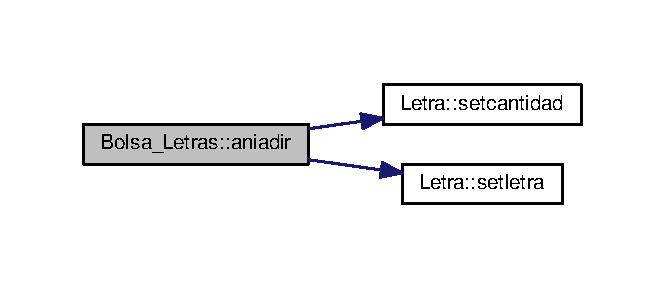
\includegraphics[width=319pt]{classBolsa__Letras_aec590e0eddf7ab585a15cda9369de21c_cgraph}
\end{center}
\end{figure}


\index{Bolsa\+\_\+\+Letras@{Bolsa\+\_\+\+Letras}!operator=@{operator=}}
\index{operator=@{operator=}!Bolsa\+\_\+\+Letras@{Bolsa\+\_\+\+Letras}}
\subsubsection[{\texorpdfstring{operator=(const Bolsa\+\_\+\+Letras \&b)}{operator=(const Bolsa_Letras &b)}}]{\setlength{\rightskip}{0pt plus 5cm}{\bf Bolsa\+\_\+\+Letras} \& Bolsa\+\_\+\+Letras\+::operator= (
\begin{DoxyParamCaption}
\item[{const {\bf Bolsa\+\_\+\+Letras} \&}]{b}
\end{DoxyParamCaption}
)}\hypertarget{classBolsa__Letras_a2c283861ab50b212023715c3959ec053}{}\label{classBolsa__Letras_a2c283861ab50b212023715c3959ec053}


\+: Operador de asignacion. 


\begin{DoxyParams}{Parámetros}
{\em } & b \+: \hyperlink{classBolsa__Letras}{Bolsa\+\_\+\+Letras} que se quiere asignar. \\
\hline
\end{DoxyParams}
\begin{DoxyReturn}{Devuelve}
\+: Devuelve una referencia al objeto. 
\end{DoxyReturn}


Definición en la línea 19 del archivo Bolsa\+\_\+\+Letras.\+cpp.


\begin{DoxyCode}
19                                                            \{
20     bolsa = b.bolsa;
21 \}
\end{DoxyCode}


\subsection{Documentación de las funciones relacionadas y clases amigas}
\index{Bolsa\+\_\+\+Letras@{Bolsa\+\_\+\+Letras}!operator$<$$<$@{operator$<$$<$}}
\index{operator$<$$<$@{operator$<$$<$}!Bolsa\+\_\+\+Letras@{Bolsa\+\_\+\+Letras}}
\subsubsection[{\texorpdfstring{operator$<$$<$}{operator<<}}]{\setlength{\rightskip}{0pt plus 5cm}ostream\& operator$<$$<$ (
\begin{DoxyParamCaption}
\item[{ostream \&}]{os, }
\item[{const {\bf Bolsa\+\_\+\+Letras} \&}]{c}
\end{DoxyParamCaption}
)\hspace{0.3cm}{\ttfamily [friend]}}\hypertarget{classBolsa__Letras_a4467ebafe1a0f889e3fda938465ed12c}{}\label{classBolsa__Letras_a4467ebafe1a0f889e3fda938465ed12c}


\+: Escribe en un flujo de salida una \hyperlink{classBolsa__Letras}{Bolsa\+\_\+\+Letras}. 


\begin{DoxyParams}{Parámetros}
{\em } & os \+: Flujo de salida. \\
\hline
{\em } & b \+: El objeto \hyperlink{classBolsa__Letras}{Bolsa\+\_\+\+Letras} que se escribe. \\
\hline
\end{DoxyParams}
\begin{DoxyReturn}{Devuelve}
\+: Flujo de salida. 
\end{DoxyReturn}


Definición en la línea 180 del archivo Bolsa\+\_\+\+Letras.\+cpp.


\begin{DoxyCode}
180                                                            \{
181     \textcolor{comment}{/*os << "#Letra\(\backslash\)t Cant\(\backslash\)t Puntuacion" << endl;}
182 \textcolor{comment}{    for (int i = 0; i < b.bolsa.size(); i++)}
183 \textcolor{comment}{        os << b.bolsa[i] << endl;}
184 \textcolor{comment}{}
185 \textcolor{comment}{    return os;*/}
186 
187     os << \textcolor{stringliteral}{"Las letras son "};
188     \textcolor{keywordflow}{for} (\textcolor{keywordtype}{int} i = 0; i < b.bolsa.size(); i++)
189         \textcolor{keywordflow}{for} (\textcolor{keywordtype}{int} j = 0; j < b.bolsa[i].getcantidad(); j++)
190             os << b.bolsa[i].getletra() << \textcolor{stringliteral}{" "};
191 
192     \textcolor{keywordflow}{return} os;
193 \}
\end{DoxyCode}
\index{Bolsa\+\_\+\+Letras@{Bolsa\+\_\+\+Letras}!operator$>$$>$@{operator$>$$>$}}
\index{operator$>$$>$@{operator$>$$>$}!Bolsa\+\_\+\+Letras@{Bolsa\+\_\+\+Letras}}
\subsubsection[{\texorpdfstring{operator$>$$>$}{operator>>}}]{\setlength{\rightskip}{0pt plus 5cm}istream\& operator$>$$>$ (
\begin{DoxyParamCaption}
\item[{istream \&}]{is, }
\item[{{\bf Bolsa\+\_\+\+Letras} \&}]{b}
\end{DoxyParamCaption}
)\hspace{0.3cm}{\ttfamily [friend]}}\hypertarget{classBolsa__Letras_a411e49a5cfaff550ca5f6977ff18efba}{}\label{classBolsa__Letras_a411e49a5cfaff550ca5f6977ff18efba}


\+: Lee de un flujo de entrada una \hyperlink{classBolsa__Letras}{Bolsa\+\_\+\+Letras}. 


\begin{DoxyParams}{Parámetros}
{\em } & is \+: Flujo de entrada. \\
\hline
{\em } & b \+: El objeto donde se realiza la lectura. \\
\hline
\end{DoxyParams}
\begin{DoxyReturn}{Devuelve}
\+: Flujo de entrada. 
\end{DoxyReturn}


Definición en la línea 170 del archivo Bolsa\+\_\+\+Letras.\+cpp.


\begin{DoxyCode}
170                                                      \{
171     \textcolor{keywordtype}{string} cabecera;
172     getline(is, cabecera);
173     \hyperlink{classLetra}{Letra} aux;
174 
175     \textcolor{keywordflow}{while}(is >> aux)
176         b.\hyperlink{classBolsa__Letras_aec590e0eddf7ab585a15cda9369de21c}{aniadir}(aux);
177 
178     \textcolor{keywordflow}{return} is;
179 \}
\end{DoxyCode}


La documentación para esta clase fue generada a partir de los siguientes ficheros\+:\begin{DoxyCompactItemize}
\item 
include/Bolsa\+\_\+\+Letras.\+h\item 
src/Bolsa\+\_\+\+Letras.\+cpp\end{DoxyCompactItemize}

\hypertarget{classDiccionario}{}\section{Referencia de la Clase Diccionario}
\label{classDiccionario}\index{Diccionario@{Diccionario}}
\subsection*{Clases}
\begin{DoxyCompactItemize}
\item 
class \hyperlink{classDiccionario_1_1iter}{iter}
\end{DoxyCompactItemize}
\subsection*{Métodos públicos}
\begin{DoxyCompactItemize}
\item 
\hyperlink{classDiccionario_aa0a2191ec706b256c35b5229cc197b15}{Diccionario} ()\hypertarget{classDiccionario_aa0a2191ec706b256c35b5229cc197b15}{}\label{classDiccionario_aa0a2191ec706b256c35b5229cc197b15}

\begin{DoxyCompactList}\small\item\em \+: Construye un diccionario vacío. \end{DoxyCompactList}\item 
int \hyperlink{classDiccionario_abe2e0023732c4cef7f6960120e8cde39}{size} () const 
\begin{DoxyCompactList}\small\item\em \+: Devuelve el numero de palabras en el diccionario. \end{DoxyCompactList}\item 
vector$<$ string $>$ \hyperlink{classDiccionario_a6ec8594ebcc112eea474ae1ff86629be}{Palabras\+Longitud} (int longitud)
\begin{DoxyCompactList}\small\item\em \+: Obtiene todas las palabras en el diccionario de una longitud dada. \end{DoxyCompactList}\item 
bool \hyperlink{classDiccionario_a2091d415bc53c34a0e78e7bd9b073024}{Esta} (string palabra)
\begin{DoxyCompactList}\small\item\em \+: Indica si una palabra esta en el diccionario o no. \end{DoxyCompactList}\item 
bool {\bfseries Generar\+Ficheros} (string letras, string frecuencias)\hypertarget{classDiccionario_a2835b073f7ed7a4e0f76ac26d8cc606e}{}\label{classDiccionario_a2835b073f7ed7a4e0f76ac26d8cc606e}

\item 
\hyperlink{classDiccionario_1_1iter}{iter} {\bfseries begin} () const \hypertarget{classDiccionario_a0a59b070ea0434b8a23afa77b0979d34}{}\label{classDiccionario_a0a59b070ea0434b8a23afa77b0979d34}

\item 
\hyperlink{classDiccionario_1_1iter}{iter} {\bfseries end} () const \hypertarget{classDiccionario_ac2a8812c73049c7ac557f7f34695da67}{}\label{classDiccionario_ac2a8812c73049c7ac557f7f34695da67}

\end{DoxyCompactItemize}
\subsection*{Amigas}
\begin{DoxyCompactItemize}
\item 
istream \& \hyperlink{classDiccionario_a940c6d9371bca891c95a5a044a42905f}{operator$>$$>$} (istream \&is, \hyperlink{classDiccionario}{Diccionario} \&D)
\begin{DoxyCompactList}\small\item\em \+: Lee de un flujo de entrada un diccionario. \end{DoxyCompactList}\item 
ostream \& \hyperlink{classDiccionario_aad8d25118e38f63c35cfc247af45a78a}{operator$<$$<$} (ostream \&os, const \hyperlink{classDiccionario}{Diccionario} \&D)
\begin{DoxyCompactList}\small\item\em \+: Escribe en un flujo de salida un diccionario. \end{DoxyCompactList}\end{DoxyCompactItemize}


\subsection{Descripción detallada}


Definición en la línea 10 del archivo Diccionario.\+h.



\subsection{Documentación de las funciones miembro}
\index{Diccionario@{Diccionario}!Esta@{Esta}}
\index{Esta@{Esta}!Diccionario@{Diccionario}}
\subsubsection[{\texorpdfstring{Esta(string palabra)}{Esta(string palabra)}}]{\setlength{\rightskip}{0pt plus 5cm}bool Diccionario\+::\+Esta (
\begin{DoxyParamCaption}
\item[{string}]{palabra}
\end{DoxyParamCaption}
)}\hypertarget{classDiccionario_a2091d415bc53c34a0e78e7bd9b073024}{}\label{classDiccionario_a2091d415bc53c34a0e78e7bd9b073024}


\+: Indica si una palabra esta en el diccionario o no. 


\begin{DoxyParams}{Parámetros}
{\em } & palabra \+: La palabra que se quiere buscar. \\
\hline
\end{DoxyParams}
\begin{DoxyReturn}{Devuelve}
\+: True si la palabra esta en el diccionario y false en caso contrario. 
\end{DoxyReturn}


Definición en la línea 27 del archivo Diccionario.\+cpp.


\begin{DoxyCode}
27                                     \{
28     \textcolor{keywordtype}{bool} resultado = \textcolor{keyword}{true};
29     \textcolor{keywordflow}{if} ( datos.find(palabra) == datos.end() )
30         resultado = \textcolor{keyword}{false};
31 
32     \textcolor{keywordflow}{return} resultado;
33 \}
\end{DoxyCode}
\index{Diccionario@{Diccionario}!Palabras\+Longitud@{Palabras\+Longitud}}
\index{Palabras\+Longitud@{Palabras\+Longitud}!Diccionario@{Diccionario}}
\subsubsection[{\texorpdfstring{Palabras\+Longitud(int longitud)}{PalabrasLongitud(int longitud)}}]{\setlength{\rightskip}{0pt plus 5cm}vector$<$ string $>$ Diccionario\+::\+Palabras\+Longitud (
\begin{DoxyParamCaption}
\item[{int}]{longitud}
\end{DoxyParamCaption}
)}\hypertarget{classDiccionario_a6ec8594ebcc112eea474ae1ff86629be}{}\label{classDiccionario_a6ec8594ebcc112eea474ae1ff86629be}


\+: Obtiene todas las palabras en el diccionario de una longitud dada. 


\begin{DoxyParams}{Parámetros}
{\em } & longitud \+: La longitud de las palabras de salida. \\
\hline
\end{DoxyParams}
\begin{DoxyReturn}{Devuelve}
\+: Vector con las palabras de la longitud especificada por el parametro. 
\end{DoxyReturn}


Definición en la línea 18 del archivo Diccionario.\+cpp.


\begin{DoxyCode}
18                                                         \{
19     vector<string> aux;
20     \textcolor{keywordflow}{for} (\textcolor{keyword}{auto} it:datos)
21         \textcolor{keywordflow}{if} (it.size() == longitud)
22             aux.push\_back(it);
23 
24     \textcolor{keywordflow}{return} aux;
25 \}
\end{DoxyCode}
\index{Diccionario@{Diccionario}!size@{size}}
\index{size@{size}!Diccionario@{Diccionario}}
\subsubsection[{\texorpdfstring{size() const }{size() const }}]{\setlength{\rightskip}{0pt plus 5cm}int Diccionario\+::size (
\begin{DoxyParamCaption}
{}
\end{DoxyParamCaption}
) const}\hypertarget{classDiccionario_abe2e0023732c4cef7f6960120e8cde39}{}\label{classDiccionario_abe2e0023732c4cef7f6960120e8cde39}


\+: Devuelve el numero de palabras en el diccionario. 

\begin{DoxyReturn}{Devuelve}
\+: Numero de palabras en el diccionario. 
\end{DoxyReturn}


Definición en la línea 14 del archivo Diccionario.\+cpp.


\begin{DoxyCode}
14                            \{
15     \textcolor{keywordflow}{return} datos.size();
16 \}
\end{DoxyCode}


\subsection{Documentación de las funciones relacionadas y clases amigas}
\index{Diccionario@{Diccionario}!operator$<$$<$@{operator$<$$<$}}
\index{operator$<$$<$@{operator$<$$<$}!Diccionario@{Diccionario}}
\subsubsection[{\texorpdfstring{operator$<$$<$}{operator<<}}]{\setlength{\rightskip}{0pt plus 5cm}ostream\& operator$<$$<$ (
\begin{DoxyParamCaption}
\item[{ostream \&}]{os, }
\item[{const {\bf Diccionario} \&}]{D}
\end{DoxyParamCaption}
)\hspace{0.3cm}{\ttfamily [friend]}}\hypertarget{classDiccionario_aad8d25118e38f63c35cfc247af45a78a}{}\label{classDiccionario_aad8d25118e38f63c35cfc247af45a78a}


\+: Escribe en un flujo de salida un diccionario. 


\begin{DoxyParams}{Parámetros}
{\em } & os \+: Flujo de salida. \\
\hline
{\em } & D \+: El objeto diccionario que se escribe. \\
\hline
\end{DoxyParams}
\begin{DoxyReturn}{Devuelve}
\+: Flujo de salida. 
\end{DoxyReturn}


Definición en la línea 141 del archivo Diccionario.\+cpp.


\begin{DoxyCode}
141                                                          \{
142     \textcolor{keywordflow}{for} (\textcolor{keyword}{auto} it:D.datos)\{
143         os << it << endl;
144     \}
145 
146     \textcolor{keywordflow}{return} os;
147 \}
\end{DoxyCode}
\index{Diccionario@{Diccionario}!operator$>$$>$@{operator$>$$>$}}
\index{operator$>$$>$@{operator$>$$>$}!Diccionario@{Diccionario}}
\subsubsection[{\texorpdfstring{operator$>$$>$}{operator>>}}]{\setlength{\rightskip}{0pt plus 5cm}istream\& operator$>$$>$ (
\begin{DoxyParamCaption}
\item[{istream \&}]{is, }
\item[{{\bf Diccionario} \&}]{D}
\end{DoxyParamCaption}
)\hspace{0.3cm}{\ttfamily [friend]}}\hypertarget{classDiccionario_a940c6d9371bca891c95a5a044a42905f}{}\label{classDiccionario_a940c6d9371bca891c95a5a044a42905f}


\+: Lee de un flujo de entrada un diccionario. 


\begin{DoxyParams}{Parámetros}
{\em } & is \+: Flujo de entrada. \\
\hline
{\em } & D \+: El objeto donde se realiza la lectura. \\
\hline
\end{DoxyParams}
\begin{DoxyReturn}{Devuelve}
\+: Flujo de entrada. 
\end{DoxyReturn}


Definición en la línea 132 del archivo Diccionario.\+cpp.


\begin{DoxyCode}
132                                                    \{
133     \textcolor{keywordtype}{string} aux;
134 
135     \textcolor{keywordflow}{while} ( getline(is, aux) )
136         D.datos.insert(aux);
137 
138     \textcolor{keywordflow}{return} is;
139 \}
\end{DoxyCode}


La documentación para esta clase fue generada a partir de los siguientes ficheros\+:\begin{DoxyCompactItemize}
\item 
include/Diccionario.\+h\item 
src/Diccionario.\+cpp\end{DoxyCompactItemize}

\hypertarget{classDiccionario_1_1iter}{}\section{Referencia de la Clase Diccionario\+:\+:iter}
\label{classDiccionario_1_1iter}\index{Diccionario\+::iter@{Diccionario\+::iter}}
\subsection*{Métodos públicos}
\begin{DoxyCompactItemize}
\item 
string {\bfseries operator$\ast$} ()\hypertarget{classDiccionario_1_1iter_a6af7a0c96a2306418a1dd6440dd59637}{}\label{classDiccionario_1_1iter_a6af7a0c96a2306418a1dd6440dd59637}

\item 
\hyperlink{classDiccionario_1_1iter}{iter} \& {\bfseries operator++} ()\hypertarget{classDiccionario_1_1iter_af4c17c367ede4317ea2628d3ac80ad0f}{}\label{classDiccionario_1_1iter_af4c17c367ede4317ea2628d3ac80ad0f}

\item 
bool {\bfseries operator==} (const \hyperlink{classDiccionario_1_1iter}{iter} \&i)\hypertarget{classDiccionario_1_1iter_a0c66656f91fc8dd2bb30ac2933b115d2}{}\label{classDiccionario_1_1iter_a0c66656f91fc8dd2bb30ac2933b115d2}

\item 
bool {\bfseries operator!=} (const \hyperlink{classDiccionario_1_1iter}{iter} \&i)\hypertarget{classDiccionario_1_1iter_a2afe32e79fd067a67e14b2769ae2fc26}{}\label{classDiccionario_1_1iter_a2afe32e79fd067a67e14b2769ae2fc26}

\end{DoxyCompactItemize}
\subsection*{Amigas}
\begin{DoxyCompactItemize}
\item 
class {\bfseries Diccionario}\hypertarget{classDiccionario_1_1iter_ad36be158dde0129b4e0d03d0e454a26b}{}\label{classDiccionario_1_1iter_ad36be158dde0129b4e0d03d0e454a26b}

\end{DoxyCompactItemize}


\subsection{Descripción detallada}


Definición en la línea 55 del archivo Diccionario.\+h.



La documentación para esta clase fue generada a partir de los siguientes ficheros\+:\begin{DoxyCompactItemize}
\item 
include/Diccionario.\+h\item 
src/Diccionario.\+cpp\end{DoxyCompactItemize}

\hypertarget{classLetra}{}\section{Referencia de la Clase Letra}
\label{classLetra}\index{Letra@{Letra}}
\subsection*{Métodos públicos}
\begin{DoxyCompactItemize}
\item 
\hyperlink{classLetra_a2e236c67e3630258c6d3d9f2a9e66709}{Letra} ()\hypertarget{classLetra_a2e236c67e3630258c6d3d9f2a9e66709}{}\label{classLetra_a2e236c67e3630258c6d3d9f2a9e66709}

\begin{DoxyCompactList}\small\item\em \+: Construye una \hyperlink{classLetra}{Letra} vacía \end{DoxyCompactList}\item 
char \hyperlink{classLetra_a94a87e5d27e65cbc29c9e3b9ec25c2ef}{getletra} () const 
\begin{DoxyCompactList}\small\item\em \+: Método observador de la letra. \end{DoxyCompactList}\item 
int \hyperlink{classLetra_a6da04e78e8394286cf344a5517eefe93}{getcantidad} () const 
\begin{DoxyCompactList}\small\item\em \+: Método observador de la cantidad. \end{DoxyCompactList}\item 
int \hyperlink{classLetra_a0d1289cbbaf1ac3cef3728169fc0635d}{getpuntos} () const 
\begin{DoxyCompactList}\small\item\em \+: Método observador de los puntos. \end{DoxyCompactList}\item 
bool \hyperlink{classLetra_a60bee0a9f4fd060146a9bc6711d728c4}{setletra} (char l)
\begin{DoxyCompactList}\small\item\em \+: Asigna un valor de letra a \hyperlink{classLetra}{Letra} si es posible. \end{DoxyCompactList}\item 
bool \hyperlink{classLetra_a89680a16e9ab48e9ed0d6dee52cae82e}{setcantidad} (int c)
\begin{DoxyCompactList}\small\item\em \+: Asigna la cantidad de veces que aparece esta letra en la bolsa. \end{DoxyCompactList}\item 
bool \hyperlink{classLetra_a472f24ed48a494a80fff9f34306fac13}{setpuntos} (int p)
\begin{DoxyCompactList}\small\item\em \+: Asigna los puntos que vale la letra. \end{DoxyCompactList}\item 
bool \hyperlink{classLetra_aabf3e986f008c943f73d8451698083c4}{operator==} (const \hyperlink{classLetra}{Letra} \&l)
\begin{DoxyCompactList}\small\item\em \+: Comprueba si dos Letras son iguales, esto es, representan la misma letra. \end{DoxyCompactList}\item 
bool \hyperlink{classLetra_a52e35828c5d6d938000777e94fa8328f}{operator!=} (const \hyperlink{classLetra}{Letra} \&l)
\begin{DoxyCompactList}\small\item\em \+: Comprueba si dos Letras son distintas, esto es, representan distintas letras. \end{DoxyCompactList}\item 
\hyperlink{classLetra}{Letra} \& \hyperlink{classLetra_ace664abba8bf62853a2fa3ea77701747}{operator=} (const \hyperlink{classLetra}{Letra} \&l)
\begin{DoxyCompactList}\small\item\em \+: Operador de asignacion. \end{DoxyCompactList}\end{DoxyCompactItemize}
\subsection*{Amigas}
\begin{DoxyCompactItemize}
\item 
istream \& \hyperlink{classLetra_a7cfdbed3a9a9638fe240a3789b77e50a}{operator$>$$>$} (istream \&is, \hyperlink{classLetra}{Letra} \&l)
\begin{DoxyCompactList}\small\item\em \+: Lee de un flujo de entrada una \hyperlink{classLetra}{Letra}. \end{DoxyCompactList}\item 
ostream \& \hyperlink{classLetra_a4573c7158ebe767aa30315296da42a3a}{operator$<$$<$} (ostream \&os, const \hyperlink{classLetra}{Letra} \&l)
\begin{DoxyCompactList}\small\item\em \+: Escribe en un flujo de salida una \hyperlink{classLetra}{Letra}. \end{DoxyCompactList}\end{DoxyCompactItemize}


\subsection{Descripción detallada}


Definición en la línea 9 del archivo Letra.\+h.



\subsection{Documentación de las funciones miembro}
\index{Letra@{Letra}!getcantidad@{getcantidad}}
\index{getcantidad@{getcantidad}!Letra@{Letra}}
\subsubsection[{\texorpdfstring{getcantidad() const }{getcantidad() const }}]{\setlength{\rightskip}{0pt plus 5cm}int Letra\+::getcantidad (
\begin{DoxyParamCaption}
{}
\end{DoxyParamCaption}
) const}\hypertarget{classLetra_a6da04e78e8394286cf344a5517eefe93}{}\label{classLetra_a6da04e78e8394286cf344a5517eefe93}


\+: Método observador de la cantidad. 

\begin{DoxyReturn}{Devuelve}
\+: Devuelve la cantidad de veces que está la \hyperlink{classLetra}{Letra} en la Bolsa. 
\end{DoxyReturn}


Definición en la línea 12 del archivo Letra.\+cpp.


\begin{DoxyCode}
12                             \{
13     \textcolor{keywordflow}{return} cantidad;
14 \}
\end{DoxyCode}
\index{Letra@{Letra}!getletra@{getletra}}
\index{getletra@{getletra}!Letra@{Letra}}
\subsubsection[{\texorpdfstring{getletra() const }{getletra() const }}]{\setlength{\rightskip}{0pt plus 5cm}char Letra\+::getletra (
\begin{DoxyParamCaption}
{}
\end{DoxyParamCaption}
) const}\hypertarget{classLetra_a94a87e5d27e65cbc29c9e3b9ec25c2ef}{}\label{classLetra_a94a87e5d27e65cbc29c9e3b9ec25c2ef}


\+: Método observador de la letra. 

\begin{DoxyReturn}{Devuelve}
\+: Devuelve la letra que se representa en \hyperlink{classLetra}{Letra}. 
\end{DoxyReturn}


Definición en la línea 8 del archivo Letra.\+cpp.


\begin{DoxyCode}
8                           \{
9     \textcolor{keywordflow}{return} letra;
10 \}
\end{DoxyCode}
\index{Letra@{Letra}!getpuntos@{getpuntos}}
\index{getpuntos@{getpuntos}!Letra@{Letra}}
\subsubsection[{\texorpdfstring{getpuntos() const }{getpuntos() const }}]{\setlength{\rightskip}{0pt plus 5cm}int Letra\+::getpuntos (
\begin{DoxyParamCaption}
{}
\end{DoxyParamCaption}
) const}\hypertarget{classLetra_a0d1289cbbaf1ac3cef3728169fc0635d}{}\label{classLetra_a0d1289cbbaf1ac3cef3728169fc0635d}


\+: Método observador de los puntos. 

\begin{DoxyReturn}{Devuelve}
\+: Devuelve los puntos que vale la letra. 
\end{DoxyReturn}


Definición en la línea 16 del archivo Letra.\+cpp.


\begin{DoxyCode}
16                           \{
17     \textcolor{keywordflow}{return} puntos;
18 \}
\end{DoxyCode}
\index{Letra@{Letra}!operator"!=@{operator"!=}}
\index{operator"!=@{operator"!=}!Letra@{Letra}}
\subsubsection[{\texorpdfstring{operator"!=(const Letra \&l)}{operator!=(const Letra &l)}}]{\setlength{\rightskip}{0pt plus 5cm}bool Letra\+::operator!= (
\begin{DoxyParamCaption}
\item[{const {\bf Letra} \&}]{l}
\end{DoxyParamCaption}
)}\hypertarget{classLetra_a52e35828c5d6d938000777e94fa8328f}{}\label{classLetra_a52e35828c5d6d938000777e94fa8328f}


\+: Comprueba si dos Letras son distintas, esto es, representan distintas letras. 


\begin{DoxyParams}{Parámetros}
{\em } & l \+: \hyperlink{classLetra}{Letra} que se quiere comparar. \\
\hline
\end{DoxyParams}
\begin{DoxyReturn}{Devuelve}
\+: Devuelve true son distintas y false si no. 
\end{DoxyReturn}


Definición en la línea 54 del archivo Letra.\+cpp.


\begin{DoxyCode}
54                                     \{
55     \textcolor{keywordflow}{if} (letra != l.letra)
56         \textcolor{keywordflow}{return} \textcolor{keyword}{true};
57     \textcolor{keywordflow}{else}
58         \textcolor{keywordflow}{return} \textcolor{keyword}{false};
59 \}
\end{DoxyCode}
\index{Letra@{Letra}!operator=@{operator=}}
\index{operator=@{operator=}!Letra@{Letra}}
\subsubsection[{\texorpdfstring{operator=(const Letra \&l)}{operator=(const Letra &l)}}]{\setlength{\rightskip}{0pt plus 5cm}{\bf Letra} \& Letra\+::operator= (
\begin{DoxyParamCaption}
\item[{const {\bf Letra} \&}]{l}
\end{DoxyParamCaption}
)}\hypertarget{classLetra_ace664abba8bf62853a2fa3ea77701747}{}\label{classLetra_ace664abba8bf62853a2fa3ea77701747}


\+: Operador de asignacion. 


\begin{DoxyParams}{Parámetros}
{\em } & l \+: \hyperlink{classLetra}{Letra} que se quiere asignar. \\
\hline
\end{DoxyParams}
\begin{DoxyReturn}{Devuelve}
\+: Devuelve una referencia al objeto. 
\end{DoxyReturn}


Definición en la línea 61 del archivo Letra.\+cpp.


\begin{DoxyCode}
61                                       \{
62     letra = l.letra;
63     cantidad = l.cantidad;
64     puntos = l.puntos;
65 
66     \textcolor{keywordflow}{return} *\textcolor{keyword}{this};
67 \}
\end{DoxyCode}
\index{Letra@{Letra}!operator==@{operator==}}
\index{operator==@{operator==}!Letra@{Letra}}
\subsubsection[{\texorpdfstring{operator==(const Letra \&l)}{operator==(const Letra &l)}}]{\setlength{\rightskip}{0pt plus 5cm}bool Letra\+::operator== (
\begin{DoxyParamCaption}
\item[{const {\bf Letra} \&}]{l}
\end{DoxyParamCaption}
)}\hypertarget{classLetra_aabf3e986f008c943f73d8451698083c4}{}\label{classLetra_aabf3e986f008c943f73d8451698083c4}


\+: Comprueba si dos Letras son iguales, esto es, representan la misma letra. 


\begin{DoxyParams}{Parámetros}
{\em } & l \+: \hyperlink{classLetra}{Letra} que se quiere comparar. \\
\hline
\end{DoxyParams}
\begin{DoxyReturn}{Devuelve}
\+: Devuelve true son iguales y false si no. 
\end{DoxyReturn}


Definición en la línea 47 del archivo Letra.\+cpp.


\begin{DoxyCode}
47                                     \{
48     \textcolor{keywordflow}{if} (letra == l.letra)
49         \textcolor{keywordflow}{return} \textcolor{keyword}{true};
50     \textcolor{keywordflow}{else}
51         \textcolor{keywordflow}{return} \textcolor{keyword}{false};
52 \}
\end{DoxyCode}
\index{Letra@{Letra}!setcantidad@{setcantidad}}
\index{setcantidad@{setcantidad}!Letra@{Letra}}
\subsubsection[{\texorpdfstring{setcantidad(int c)}{setcantidad(int c)}}]{\setlength{\rightskip}{0pt plus 5cm}bool Letra\+::setcantidad (
\begin{DoxyParamCaption}
\item[{int}]{c}
\end{DoxyParamCaption}
)}\hypertarget{classLetra_a89680a16e9ab48e9ed0d6dee52cae82e}{}\label{classLetra_a89680a16e9ab48e9ed0d6dee52cae82e}


\+: Asigna la cantidad de veces que aparece esta letra en la bolsa. 


\begin{DoxyParams}{Parámetros}
{\em } & c \+: Numero de veces que se quiere quqe aparezca (debe ser mayor o igual a 1). \\
\hline
\end{DoxyParams}
\begin{DoxyReturn}{Devuelve}
\+: Devuelve true si la cantidad se ha asignado y false de lo contrario. 
\end{DoxyReturn}


Definición en la línea 29 del archivo Letra.\+cpp.


\begin{DoxyCode}
29                             \{
30     \textcolor{keywordflow}{if} (c > 0)\{
31         cantidad = c;
32         \textcolor{keywordflow}{return} \textcolor{keyword}{true};
33     \}
34     \textcolor{keywordflow}{else}
35         \textcolor{keywordflow}{return} \textcolor{keyword}{false};
36 \}
\end{DoxyCode}
\index{Letra@{Letra}!setletra@{setletra}}
\index{setletra@{setletra}!Letra@{Letra}}
\subsubsection[{\texorpdfstring{setletra(char l)}{setletra(char l)}}]{\setlength{\rightskip}{0pt plus 5cm}bool Letra\+::setletra (
\begin{DoxyParamCaption}
\item[{char}]{l}
\end{DoxyParamCaption}
)}\hypertarget{classLetra_a60bee0a9f4fd060146a9bc6711d728c4}{}\label{classLetra_a60bee0a9f4fd060146a9bc6711d728c4}


\+: Asigna un valor de letra a \hyperlink{classLetra}{Letra} si es posible. 


\begin{DoxyParams}{Parámetros}
{\em } & l \+: letra que se quiere asignar (para ello debe ir de la a ... z). \\
\hline
\end{DoxyParams}
\begin{DoxyReturn}{Devuelve}
\+: Devuelve true si la letra se ha asignado y false de lo contrario. 
\end{DoxyReturn}


Definición en la línea 20 del archivo Letra.\+cpp.


\begin{DoxyCode}
20                           \{
21     \textcolor{keywordflow}{if} ( \textcolor{charliteral}{'a'} <= l && l <= \textcolor{charliteral}{'z'})\{
22         letra = l;
23         \textcolor{keywordflow}{return} \textcolor{keyword}{true};
24     \}
25     \textcolor{keywordflow}{else}
26         \textcolor{keywordflow}{return} \textcolor{keyword}{false};
27 \}
\end{DoxyCode}
\index{Letra@{Letra}!setpuntos@{setpuntos}}
\index{setpuntos@{setpuntos}!Letra@{Letra}}
\subsubsection[{\texorpdfstring{setpuntos(int p)}{setpuntos(int p)}}]{\setlength{\rightskip}{0pt plus 5cm}bool Letra\+::setpuntos (
\begin{DoxyParamCaption}
\item[{int}]{p}
\end{DoxyParamCaption}
)}\hypertarget{classLetra_a472f24ed48a494a80fff9f34306fac13}{}\label{classLetra_a472f24ed48a494a80fff9f34306fac13}


\+: Asigna los puntos que vale la letra. 


\begin{DoxyParams}{Parámetros}
{\em } & p \+: Puntos que se quiere que valga (debe ser mayor o igual a 1). \\
\hline
\end{DoxyParams}
\begin{DoxyReturn}{Devuelve}
\+: Devuelve true si los puntos se han asignado y false de lo contrario. 
\end{DoxyReturn}


Definición en la línea 38 del archivo Letra.\+cpp.


\begin{DoxyCode}
38                           \{
39     \textcolor{keywordflow}{if} (p > 0)\{
40         puntos = p;
41         \textcolor{keywordflow}{return} \textcolor{keyword}{true};
42     \}
43     \textcolor{keywordflow}{else}
44         \textcolor{keywordflow}{return} \textcolor{keyword}{false};
45 \}
\end{DoxyCode}


\subsection{Documentación de las funciones relacionadas y clases amigas}
\index{Letra@{Letra}!operator$<$$<$@{operator$<$$<$}}
\index{operator$<$$<$@{operator$<$$<$}!Letra@{Letra}}
\subsubsection[{\texorpdfstring{operator$<$$<$}{operator<<}}]{\setlength{\rightskip}{0pt plus 5cm}ostream\& operator$<$$<$ (
\begin{DoxyParamCaption}
\item[{ostream \&}]{os, }
\item[{const {\bf Letra} \&}]{l}
\end{DoxyParamCaption}
)\hspace{0.3cm}{\ttfamily [friend]}}\hypertarget{classLetra_a4573c7158ebe767aa30315296da42a3a}{}\label{classLetra_a4573c7158ebe767aa30315296da42a3a}


\+: Escribe en un flujo de salida una \hyperlink{classLetra}{Letra}. 


\begin{DoxyParams}{Parámetros}
{\em } & os \+: Flujo de salida. \\
\hline
{\em } & D \+: El objeto \hyperlink{classLetra}{Letra} que se escribe. \\
\hline
\end{DoxyParams}
\begin{DoxyReturn}{Devuelve}
\+: Flujo de salida. 
\end{DoxyReturn}


Definición en la línea 77 del archivo Letra.\+cpp.


\begin{DoxyCode}
77                                                    \{
78     os << l.letra << \textcolor{stringliteral}{"\(\backslash\)t"} << l.cantidad << \textcolor{stringliteral}{"\(\backslash\)t"} << l.puntos;
79 \}
\end{DoxyCode}
\index{Letra@{Letra}!operator$>$$>$@{operator$>$$>$}}
\index{operator$>$$>$@{operator$>$$>$}!Letra@{Letra}}
\subsubsection[{\texorpdfstring{operator$>$$>$}{operator>>}}]{\setlength{\rightskip}{0pt plus 5cm}istream\& operator$>$$>$ (
\begin{DoxyParamCaption}
\item[{istream \&}]{is, }
\item[{{\bf Letra} \&}]{l}
\end{DoxyParamCaption}
)\hspace{0.3cm}{\ttfamily [friend]}}\hypertarget{classLetra_a7cfdbed3a9a9638fe240a3789b77e50a}{}\label{classLetra_a7cfdbed3a9a9638fe240a3789b77e50a}


\+: Lee de un flujo de entrada una \hyperlink{classLetra}{Letra}. 


\begin{DoxyParams}{Parámetros}
{\em } & is \+: Flujo de entrada. \\
\hline
{\em } & l \+: El objeto donde se realiza la lectura. \\
\hline
\end{DoxyParams}
\begin{DoxyReturn}{Devuelve}
\+: Flujo de entrada. 
\end{DoxyReturn}


Definición en la línea 69 del archivo Letra.\+cpp.


\begin{DoxyCode}
69                                              \{
70     is >> l.letra;
71     is >> l.cantidad;
72     is >> l.puntos;
73 
74     \textcolor{keywordflow}{return} is;
75 \}
\end{DoxyCode}


La documentación para esta clase fue generada a partir de los siguientes ficheros\+:\begin{DoxyCompactItemize}
\item 
include/Letra.\+h\item 
src/Letra.\+cpp\end{DoxyCompactItemize}

%--- End generated contents ---

% Index
\backmatter
\newpage
\phantomsection
\clearemptydoublepage
\addcontentsline{toc}{chapter}{Índice}
\printindex

\end{document}
